\documentclass[svgnames,11pt]{beamer}
\input{/home/tof/Documents/Cozy/latex-include/preambule_commun.tex}
\input{/home/tof/Documents/Cozy/latex-include/preambule_beamer.tex}
%\usepackage{pgfpages} \setbeameroption{show notes on second screen=left}
\author[]{Christophe Viroulaud}
\title{TP rotation image}
\date{\framebox{\textbf{Algo 03}}}
%\logo{}
\institute{Terminale - NSI}

\begin{document}
\begin{frame}
    \titlepage
\end{frame}
\begin{frame}
    \frametitle{}

    La rotation d'une image est une fonctionnalité proposée par n'importe quel logiciel de retouche tel \emph{Gimp}. L'opération n'est cependant pas triviale et peut demander une durée non négligeable.

\end{frame}
\begin{frame}
    \frametitle{}

    \begin{framed}\centering
        Construire un algorithme de rotation d'une image en appliquant le principe de \emph{diviser pour régner}.
    \end{framed}

\end{frame}
\section{Principe}
\begin{frame}
    \frametitle{Principe}

    \emph{Diviser pour régner} se décompose en trois parties:
    \begin{itemize}
        \item \emph{diviser:} Le problème est partagé en plusieurs petits problèmes identiques.
        \item \emph{traitement:} Chaque petit problème est résolu.
        \item \emph{recombinaison:} Les petits problèmes résolus sont assemblés pour remonter au problème principal.
    \end{itemize}

\end{frame}
\begin{frame}
    \frametitle{}

    \begin{activite}
        \textbf{Réflexion commune:} Considérons une image aux dimensions connues. Quelles étapes pourrions-nous imaginer pour répondre à notre problématique?
    \end{activite}

\end{frame}
\begin{frame}
    \frametitle{Avant de regarder la correction}
    \begin{center}
        \centering
        \includegraphics[width=3cm]{/home/tof/Documents/Cozy/latex-include/stop.png}
    \end{center}
    {\Large
    \begin{itemize}
        \item Prendre le temps de réfléchir,
        \item Analyser les messages d'erreur,
        \item Demander au professeur.
    \end{itemize}
    }
\end{frame}
\begin{frame}
    \frametitle{Correction}

    \begin{center}
        \centering
        
\includegraphics[width=2cm]{ressources/carre0.png}
        \captionof{figure}{1 pixel: rien à faire}
        \label{IMG}
    \end{center}

\end{frame}
\begin{frame}
    \frametitle{Correction}

    \begin{center}
        \begin{tabular}{ccc}
            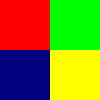
\includegraphics[width=3cm]{ressources/carre1.png}
             & $$\rightarrow$$
             &
            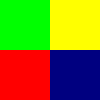
\includegraphics[width=3cm]{ressources/carre1-rot.png}
            \\
        \end{tabular}
        \captionof{figure}{Rotation}
    \end{center}
\note{pixel(l=0, c=0) $\rightarrow$ (l=1, c=0)}
\end{frame}
\begin{frame}
    \frametitle{Correction}

    \begin{center}
        \begin{tabular}{ccccc}
            
\includegraphics[width=2.5cm]{ressources/carre2.png}
             & $$\rightarrow$$
             &
            
\includegraphics[width=2.5cm]{ressources/carre2-int.png}
            & $$\rightarrow$$
             &
            
\includegraphics[width=2.5cm]{ressources/carre2-rot.png}
            \\
        \end{tabular}
        \captionof{figure}{Récursivité: on divise la taille des problèmes par 2.}
    \end{center}

\end{frame}
\begin{frame}
    \frametitle{}

    \begin{itemize}
        \item Si la taille \texttt{\textbf{t}} est égal à 1, ne rien faire.
        \item Sinon: \textbf{découper en sous problèmes}
        \begin{itemize}
            \item diviser la taille \textbf{\texttt{t}} en 2,
            \item effectuer récursivement la rotation des \textbf{quatre parties} de la portion carrée comprise entre (x,y) et (x+t, y+t)
        \end{itemize}
        \item \textbf{résoudre les petits problèmes:} Effectuer la rotation des pixels.
    \end{itemize}

\end{frame}
\section{Algorithme de rotation}
\subsection{Chargement de l'image}
\begin{frame}[fragile]
    \frametitle{Chargement de l'image}

    \emph{PIL (Python Image Library) -anciennement pillow-} est une bibliothèque de traitement d'image. 
\begin{center}
\begin{lstlisting}[language=Python , basicstyle=\ttfamily\small, xleftmargin=2em, xrightmargin=2em]
from PIL import Image

im = Image.open("image.png")
im.show()
\end{lstlisting}
\captionof{code}{Charger une image}
\label{CODE}
\end{center}  

\end{frame}
\begin{frame}[fragile]
    \frametitle{}

\begin{center}
\begin{lstlisting}[language=Python , basicstyle=\ttfamily\small, xleftmargin=2em, xrightmargin=2em]
largeur, hauteur = im.size
px = im.load()
\end{lstlisting}
\captionof{code}{Récupérer des informations}
\label{CODE}
\end{center}
\begin{aretenir}[Information]
    La variable \textbf{\texttt{px}} contient une matrice représentative des pixels de l'image. La couleur du pixel de coordonnées \textbf{\texttt{(x,y)}} est donnée par l'instruction \texttt{\textbf{px[x,y]}}. Il est également possible d'affecter une nouvelle couleur \textbf{\texttt{c}} à un pixel: \texttt{\textbf{px[x,y] = c}}.
\end{aretenir}
\end{frame}
\begin{frame}
    \frametitle{}

    \begin{activite}
        \begin{enumerate}
            \item Récupérer une image carrée sur \url{https://www.freepng.fr/}.
            \item Charger et afficher cette image.
        \end{enumerate}
        \end{activite}

\end{frame}
\subsection{Résoudre un petit problème}
\begin{frame}
    \frametitle{Résoudre un petit problème}
    \begin{center}
        \begin{tabular}{cccc}
            {\Large $t=1$}
            &
            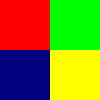
\includegraphics[width=2cm]{ressources/carre1.png}
             & $$\rightarrow$$
             &
            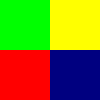
\includegraphics[width=2cm]{ressources/carre1-rot.png}
            \\
        \end{tabular}
    \end{center}
    \begin{center}
        \begin{tabular}{cccc}
            {\Large $t=2$}
            &
            
\includegraphics[width=2cm]{ressources/carre2-int.png}
            & $$\rightarrow$$
             &
            
\includegraphics[width=2cm]{ressources/carre2-rot.png}
            \\
        \end{tabular}
    \end{center}
    \begin{activite}
    Écrire la fonction \textbf{\texttt{tourner(px: object, x: int, y: int, t: int) $\rightarrow$ None}} qui effectue une rotation anti-horaire pour les pixels compris dans l'intervalle de colonnes $[x; x+t]$ et l'intervalle de lignes $[y; y+t]$.
    \end{activite}

\end{frame}
\end{document}